\documentclass[11pt,pdftex,mathserif]{beamer}\usepackage[]{graphicx}\usepackage[]{color}
%% maxwidth is the original width if it is less than linewidth
%% otherwise use linewidth (to make sure the graphics do not exceed the margin)
\makeatletter
\def\maxwidth{ %
  \ifdim\Gin@nat@width>\linewidth
    \linewidth
  \else
    \Gin@nat@width
  \fi
}
\makeatother

\definecolor{fgcolor}{rgb}{0.345, 0.345, 0.345}
\newcommand{\hlnum}[1]{\textcolor[rgb]{0.686,0.059,0.569}{#1}}%
\newcommand{\hlstr}[1]{\textcolor[rgb]{0.192,0.494,0.8}{#1}}%
\newcommand{\hlcom}[1]{\textcolor[rgb]{0.678,0.584,0.686}{\textit{#1}}}%
\newcommand{\hlopt}[1]{\textcolor[rgb]{0,0,0}{#1}}%
\newcommand{\hlstd}[1]{\textcolor[rgb]{0.345,0.345,0.345}{#1}}%
\newcommand{\hlkwa}[1]{\textcolor[rgb]{0.161,0.373,0.58}{\textbf{#1}}}%
\newcommand{\hlkwb}[1]{\textcolor[rgb]{0.69,0.353,0.396}{#1}}%
\newcommand{\hlkwc}[1]{\textcolor[rgb]{0.333,0.667,0.333}{#1}}%
\newcommand{\hlkwd}[1]{\textcolor[rgb]{0.737,0.353,0.396}{\textbf{#1}}}%

\usepackage{framed}
\makeatletter
\newenvironment{kframe}{%
 \def\at@end@of@kframe{}%
 \ifinner\ifhmode%
  \def\at@end@of@kframe{\end{minipage}}%
  \begin{minipage}{\columnwidth}%
 \fi\fi%
 \def\FrameCommand##1{\hskip\@totalleftmargin \hskip-\fboxsep
 \colorbox{shadecolor}{##1}\hskip-\fboxsep
     % There is no \\@totalrightmargin, so:
     \hskip-\linewidth \hskip-\@totalleftmargin \hskip\columnwidth}%
 \MakeFramed {\advance\hsize-\width
   \@totalleftmargin\z@ \linewidth\hsize
   \@setminipage}}%
 {\par\unskip\endMakeFramed%
 \at@end@of@kframe}
\makeatother

\definecolor{shadecolor}{rgb}{.97, .97, .97}
\definecolor{messagecolor}{rgb}{0, 0, 0}
\definecolor{warningcolor}{rgb}{1, 0, 1}
\definecolor{errorcolor}{rgb}{1, 0, 0}
\newenvironment{knitrout}{}{} % an empty environment to be redefined in TeX

\usepackage{alltt}
% ewentualnie (w trakcie przygotowania prezentacji):
% \documentclass[...,handout]{beamer} % jedna 'frame' == jeden slajd
\usepackage[T1]{polski}        % jeśli po angielsku, to skasuj
\usepackage[polish]{babel}     % jeśli po angielsku, to skasuj
\selectlanguage{polish}        % jeśli po angielsku, to skasuj
\usepackage[T1]{fontenc}
\usepackage[utf8]{inputenc}  % kodowanie polskich znaków CP1250 (windows)
% Alternatywnie - latin2 dla kodowania ISO-8859-2 (raczej nie Windows)
% latex/pdflatex nie wspiera niestety Unicode (np. UTF-8)
\usepackage{amsmath,amssymb}     % więcej symboli matematycznych
\usepackage{graphicx}            % jeśli chcemy wstawiać grafikę
\usepackage{hyperref}            % odnośniki internetowe, zaawansowane ust. PDF
%\hypersetup{pdfstartview={FitW}}
\usepackage{natbib}
%%%%%%%%%%%% MOJE ULUBIONE USTAWIENIA BEAMERA %%%%%%%%%%%%%
%
\usetheme{Boadilla} % Warsaw to nazwa stylu - zmień na SWOJĄ ulubioną
\usecolortheme{spruce}
\useoutertheme{infolines}
\useinnertheme{circles}
\usefonttheme{structuresmallcapsserif}
%%
\setbeamertemplate{navigation symbols}{} % WYŁĄCZA PASEK NAWIGACJI U DOŁU
\setbeamercovered{invisible} % WPŁYWA NA WYŚWIETLANIE "SPAUZOWANYCH" ELEMENTÓW

%
\setbeamertemplate{theorems}[numbered]
\definecolor{green2}{rgb}{0.3, 0.6 ,0.4}
%
%%%%%%%%%%%%%%%%%%%%%%%%%%%%%%%%%%%%%%%%%%%%%%%%%%%%%%%%%%%
%
\title[Abraham Wald]{Abraham Wald}
\author[N. Potocka]{Natalia Potocka}
%\institute[MiNI PW]{}
\date[21.04.2015]{21.04.2015}
%
%%%%%%%%%%%%%%%%%%%%%%%%%%%%%%%%%%%%%%%%%%%%%%%%%%%%%%%%%%%
%
\newtheorem{twierdzenie}{Twierdzenie}
\renewcommand{\proofname}{Dowód}
\newtheorem{lemat}[twierdzenie]{Lemat}
\newtheorem{wniosek}[twierdzenie]{Wniosek}
\newtheorem{stwierdzenie}[twierdzenie]{Stwierdzenie}

\theoremstyle{definition}
\newtheorem*{definicja}{Definicja}
\newtheorem*{oznaczenie}{Oznaczenie}

\newcommand{\R}{\mathbb{R}}
\newcommand{\N}{\mathbb{N}}
\newcommand{\E}{\mathbb{E}}
\newcommand{\xsr}{\overline{X}_n}
\newcommand{\skw}{S_n^2}
\newcommand{\al}{\alpha}
\newcommand*{\om}{\omega}


\newenvironment{zrodlo}{\emph{Źródło: }}{\par}
\IfFileExists{upquote.sty}{\usepackage{upquote}}{}
\begin{document}   % jedziemy :-)
%%%%%%%%%%%%% SLAJD TYTUŁOWY %%%%%%%%%%%%%%%%%%%%%%%%%%%%%%%%%%%%%%%%%%%%%
\thispagestyle{empty}% wyłącza paski na górze i na dole
\begin{frame}%

   \begin{center}%
%
%
%   %%%%%%%%%%%% NAGLOWEK %%%%%%%%%%%%%%%%%%%%%%%%%%%%%%%%%%%%%%%%%%%%%%%
%
      \begin{columns}%
         \begin{column}[c]{1.2cm}\centering%
         
\includegraphics[height=1.0cm]{logopw.pdf} \\%
         \end{column}

         \begin{column}[c]{7cm}\centering
            {\footnotesize{Politechnika Warszawska}}\\%
            {\footnotesize{Wydział Matematyki i~Nauk Informacyjnych}}%
         \end{column}

         \begin{column}[c]{1.2cm}\centering%
         
\includegraphics[height=1.0cm]{logomini.pdf} \\%
         \end{column}%
      \end{columns}

   %%%%%%%% TYTUL %%%%%%%%%%%%%%%%%%%%%%%%%%%%%%%%%%%%%%%%%%%%%%%%%%%%%%

      \vspace*{2em}

      \colorbox{green2}{\parbox{10cm}{\color{black}\centering\LARGE{Abraham Wald}}}

      \vspace*{1.5em}%
      {\Large{Natalia Potocka}}\\%
%      {\color{blue}\footnotesize\texttt{M.Gagolewski@mini.pw.edu.pl}}

      %\vspace*{2.5em}%
      {\it\footnotesize Warszawa, 21.04.2014}  % DATA

   \end{center}

\end{frame}

%%%%%%%%%%%%%%%%%%%CZESC NATALII%%%%%%%%%%%%%%%%%%%%%%%%%%%%%%%%%%%%%%%%%%



\begin{frame}{Pochodzenie}
\begin{itemize}
\item urodzony 31 października 1902 w Kolozsvdar (Austrowęgry, obecnie Cluj w Rumunii)
\item żydowska rodzina, syn biznesmena, wnuk rabina
\item pięcioro rodzeństwa
\item prawie cała rodzina zginęła w niemieckich obozach koncentracyjnych
\end{itemize}
\end{frame}


\begin{frame}{Wczesne lata}
Wald nie uczęszczał do~szkoły, gdyż z~powodów religijnych nie mógł chodzić do~niej w~soboty. Uczyli go~rodzice aż~do~czasu college'u. Dostał się do~Universytetu w Cluj. Z~powodu restrykcji Żydów w tym czasie, nie dostał się do~Uniwersytetu Wiedeńskiego. Uczył się więc przez rok w~szkole inżynierskiej w~Wiedniu. \pause Ostatecznie dostał się na~Uniwersytet Wiedeński w~1927, gdzie pracował z~Karlem Mengerem. Doktorat zdobył w~1931 roku. Ponieważ w~latach 30-tych XX w. podjęcie pracy na~Uniwersytecie dla Żyda było wyjątkowo trudne, podjął on~pracę dla czołowego w~tamtych czasach bankiera i~ekonomistę austriackiego, Karla Schlesingera, równocześnie wciąż się ucząc. \pause Między 1931 a~1937 napisał razem z~Mengerem 21 artykułów z~geometrii i 10 artykułów z~ekonomii i~ekonometrii.
\end{frame}


\begin{frame}{Dalsza kariera w USA}
W~sierpniu 1938 roku Wald wyjechał do~Stanów Zjednoczonych na~zaproszenie Cowles Commission. Od~września 1938 został pracownikiem Carnegie Corporation i~równocześnie studiował statystykę na~Uniwersytecie Columbia w~Nowym Jorku pod nadzorem Harolda Hotellinga. Rok ten uważa się za~jeden z najpłodniejszych pod względem jego odkryć. Wtedy właśnie zdefiniował funkcję straty, funkcję ryzyka, rozkład a priori, reguły decyzyjne Bayesa oraz reguły minimaxu.\\ \pause
Od 1939 roku został wykładowcą na~Uniwersytecie Columbia, a~od~1941 był członkiem ciała akademickiego, którym pozostał do~swojej śmierci. W~czasie wojny pracował przy projektach militarnych m.in. opracowując plan wzmocnienia samolotów.\\ \pause
W~1941 roku żeni się z~Lucille Lang. Mają razem dwójkę dzieci: Betty i~Roberta (później znany fizyk).
\end{frame}


\begin{frame}{Indie}
\begin{columns}
  \begin{column}{0.49\textwidth}
W~listopadzie 1950 roku Wald wyjeżdża do~Indii na~zaproszenie władz tego kraju, na objazd po~indyjskich uniwersytetach i~centrach badawczych. Miał uczyć swojej nowej teorii na~tamtejszych uczelniach. Niestety, 13 grudnia 1950 roku samolot linii Air India, z~powodu mgły, rozbił się na~górze Nilgris, zabijając wszystkich na~pokładzie, w~tym państwo Wald.
  \end{column}
  \begin{column}{0.49\textwidth}
  \begin{figure}
    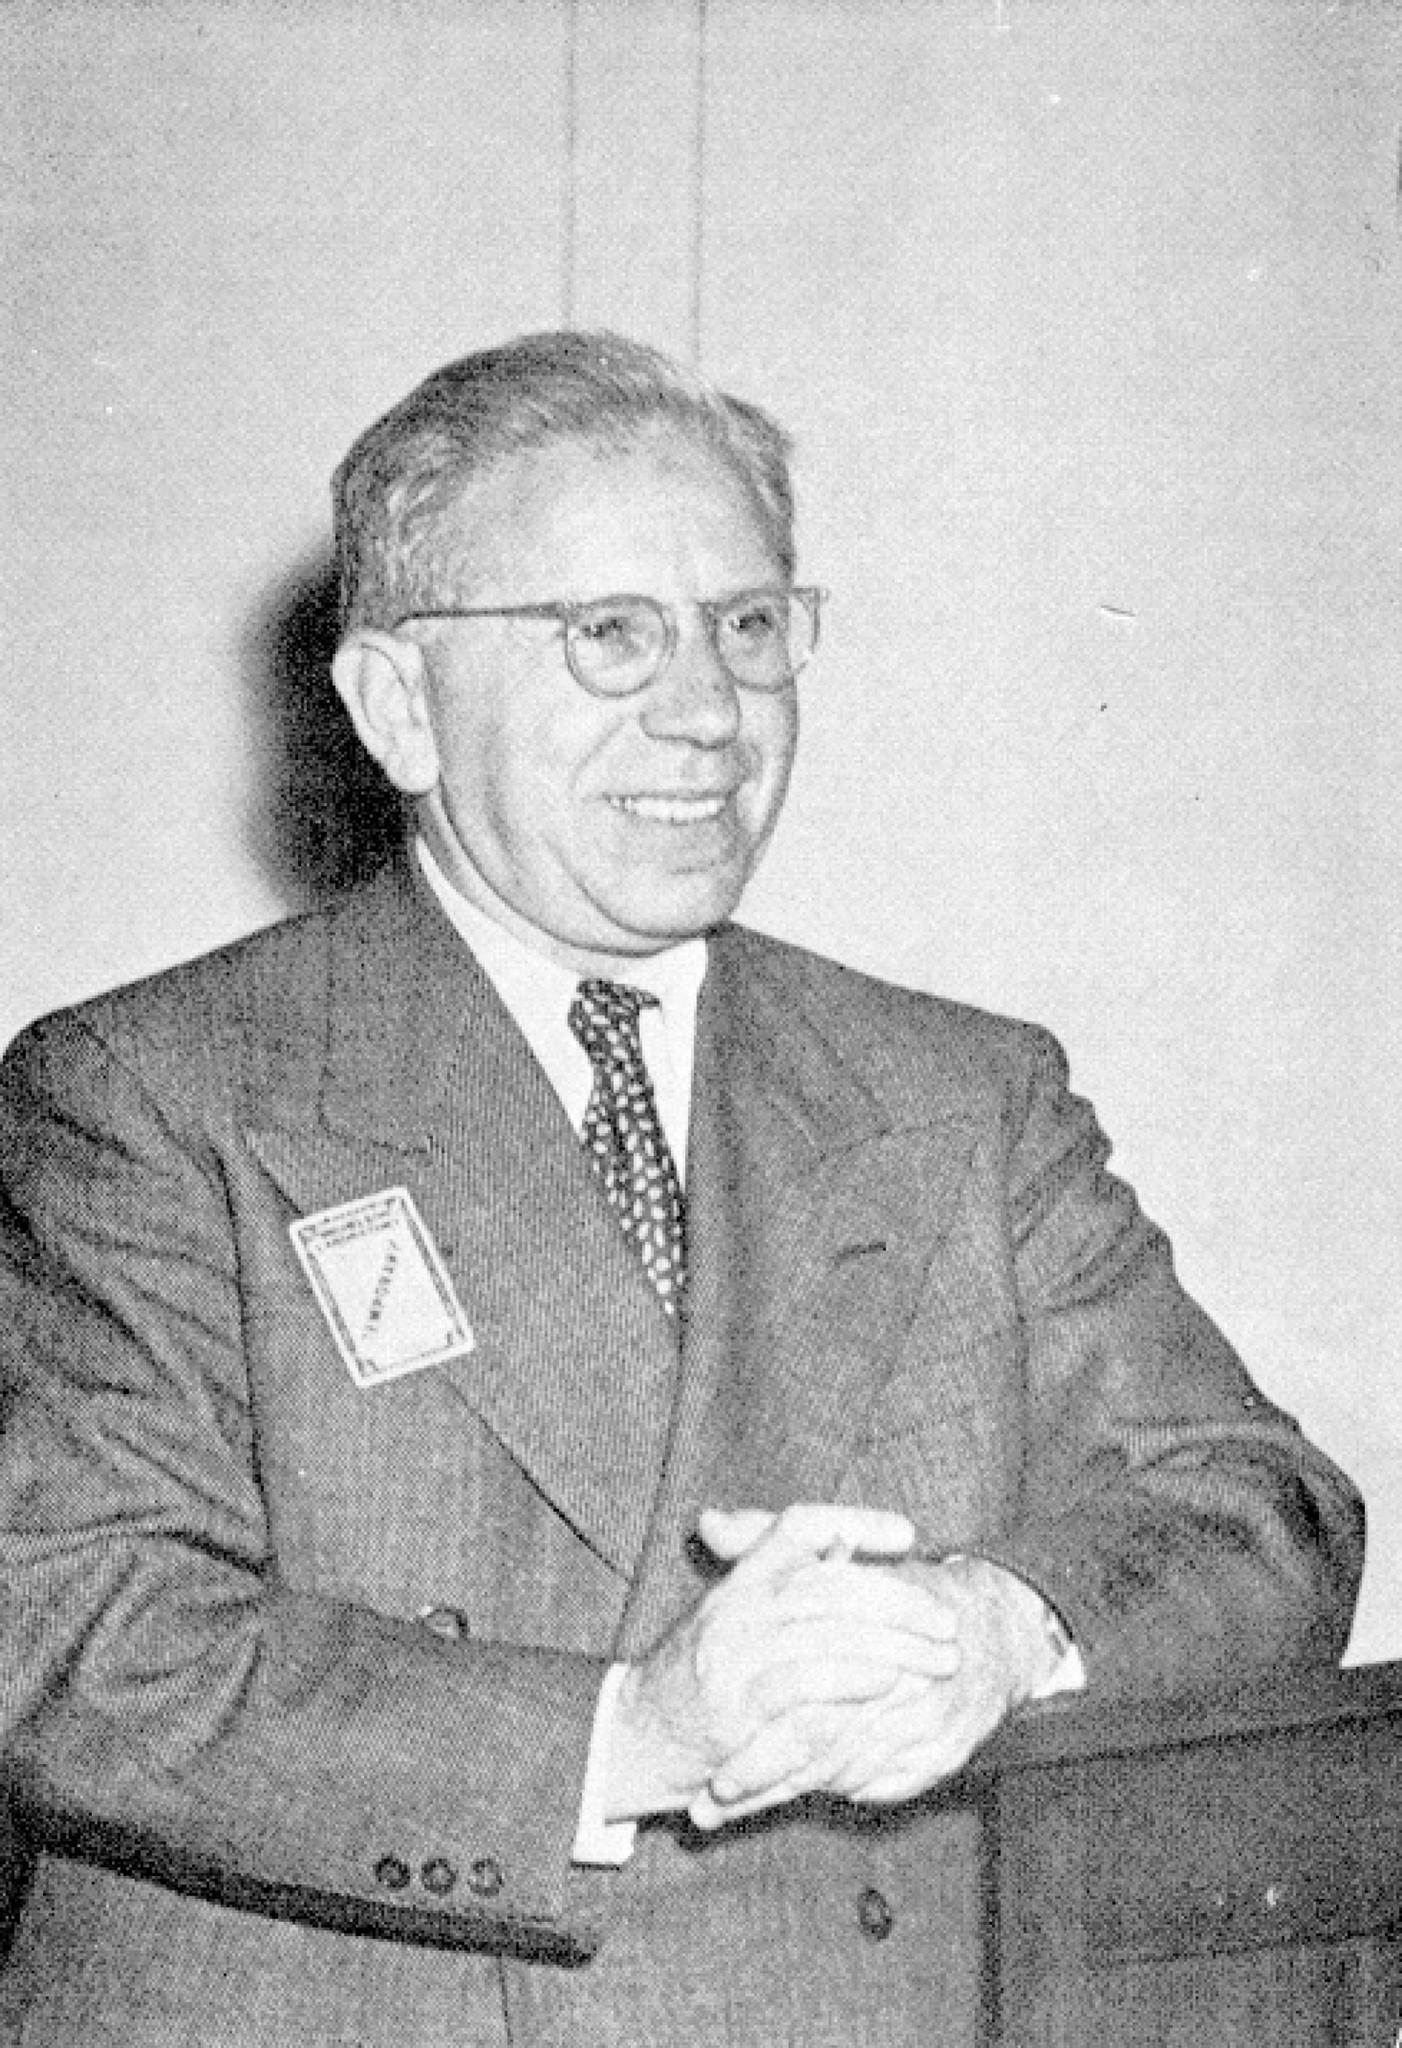
\includegraphics[width=5cm]{wald1.jpg}
  \end{figure}
\end{column}
\end{columns}
\end{frame}



\begin{frame}{Czym się zajmował}
W obszarze zainteresowań Walda były takie dziedziny jak:
\begin{itemize}
\item geometria
\item ekonomia
\item ekonometria
\item statystyka
\end{itemize}
\end{frame}



\begin{frame}{Skąd go znamy?}
\begin{itemize}
\item statystyczna teoria decyzyjna
\item analiza sekwencyjna
\item test Walda $$H_0: \theta = \theta_0,\ H_1: \theta \neq \theta_0 $$ $$\Rightarrow \frac{(\widehat{\theta} - \theta_0)^2}{Var(\widehat{\theta})} \sim \chi^2 $$
\item test serii 
\item odwrócony rozkład Gamma (znany również jako rozkład Walda) $$ f(x,\mu,\lambda) = \frac{\lambda}{2\pi x^3}exp\frac{-\lambda(x-\mu)^2}{2\mu x} $$
\item równanie Walda $$\E[X_1 + \ldots + X_N] = \E[N]\E[X_1]$$
\end{itemize}
\end{frame}


\begin{frame}{Bibliografia}
\nocite{Wolfowitz1951:wald}
\nocite{Hist:wald}
\nocite{Enc:wald}
\bibliographystyle{plain}
\bibliography{wald_bib}
\end{frame}


% \begin{frame}{Bibliografia}
% 
% \begin{thebibliography}{}
% \bibitem[1]{AS} Ananda Sen, \textit{On the Interrelation Between the Sample Mean and Sample Variance}, The American Statistician, 66 (2012), 112-117.
% %\bibitem[2]{CZ} L. N. de Castro, F. J. Von Zuben, "\href{http://www.dca.fee.unicamp.br/~vonzuben/research/lnunes_dout/artigos/gecco00.pdf}{\textit{The Clonal Selection Algorithm with Engineering Applications}}", GECCO 2000, Workshop on
% %        Artificial Immune Systems and Their Applications, Las Vegas, USA, str.
% %        36-37, 2000.
% %\bibitem[3]{M} \href{http://mst.mimuw.edu.pl/lecture.php?lecture=mbm&part=Ch12}{http://mst.mimuw.edu.pl/lecture.php?lecture=mbm&part=Ch12}
% %\bibitem[4]{IPIPAN} \href{www.ipipan.waw.pl/\~{}stw/ais/daaisy.html}{www.ipipan.waw.pl/\~{}stw/ais/daaisy.html}
% 
% 
% 
% \end{thebibliography}
% \end{frame}

\begin{frame}{}
   \begin{center}
      \Huge{Dziękuję za uwagę.}
   \end{center}
\end{frame}



\end{document}
